\documentclass[aspectratio=169]{beamer}

\mode<presentation>

\usepackage[utf8]{inputenc}
\usepackage[T1]{fontenc}	%makes å,ä,ö etc. proper symbols
\usepackage{amsmath}
\usepackage{graphicx}
\usepackage{xcolor}
\usepackage{listings}
\usepackage{multicol}
\usepackage{hyperref}
\usepackage[swedish]{babel}

\definecolor{LundaGroen}{RGB}{00,68,71}
\definecolor{StabilaLila}{RGB}{85,19,78}
\definecolor{VarmOrange}{RGB}{237,104,63}

\definecolor{MagnoliaRosa}{RGB}{251,214,209}
\definecolor{LundaHimmel}{RGB}{204,225,225}
\definecolor{LundaLjus}{RGB}{255,242,191}

\usefonttheme{serif}
\usetheme{malmoe}
\setbeamercolor{palette primary}{bg=LundaHimmel, fg=StabilaLila}
\setbeamercolor{palette quaternary}{bg=LundaGroen, fg=MagnoliaRosa}
\setbeamercolor{background canvas}{bg=LundaLjus}
\setbeamercolor{structure}{fg=LundaGroen}

\usepackage[many]{tcolorbox}

\newtcolorbox{cross}{blank,breakable,parbox=false,
  overlay={\draw[red,line width=5pt] (interior.south west)--(interior.north east);
    \draw[red,line width=5pt] (interior.north west)--(interior.south east);}}
    
\newcommand{\code}[1]{\colorbox{white}{\lstinline{#1}}}



\lstset{language=Python} 
\lstset{%language=[LaTeX]Tex,%C++,
    morekeywords={PassOptionsToPackage,selectlanguage,True,False},
    keywordstyle=\color{blue},%\bfseries,
    basicstyle=\small\ttfamily,
    %identifierstyle=\color{NavyBlue},
    commentstyle=\color{red}\ttfamily,
    stringstyle=\color{VarmOrange},
    numbers=left,%
    numberstyle=\scriptsize,%\tiny
    stepnumber=1,
    numbersep=8pt,
    showstringspaces=false,
    breaklines=true,
    %frameround=ftff,
    frame=single,
    belowcaptionskip=.75\baselineskip,
	tabsize=4,
	backgroundcolor=\color{white}
    %frame=L
}
\lstset{
	escapeinside={(*@}{@*)}
}
\begin{document}

\lstset{literate=
  {á}{{\'a}}1 {é}{{\'e}}1 {í}{{\'i}}1 {ó}{{\'o}}1 {ú}{{\'u}}1
  {Á}{{\'A}}1 {É}{{\'E}}1 {Í}{{\'I}}1 {Ó}{{\'O}}1 {Ú}{{\'U}}1
  {à}{{\`a}}1 {è}{{\`e}}1 {ì}{{\`i}}1 {ò}{{\`o}}1 {ù}{{\`u}}1
  {À}{{\`A}}1 {È}{{\'E}}1 {Ì}{{\`I}}1 {Ò}{{\`O}}1 {Ù}{{\`U}}1
  {ä}{{\"a}}1 {ë}{{\"e}}1 {ï}{{\"i}}1 {ö}{{\"o}}1 {ü}{{\"u}}1
  {Ä}{{\"A}}1 {Ë}{{\"E}}1 {Ï}{{\"I}}1 {Ö}{{\"O}}1 {Ü}{{\"U}}1
  {â}{{\^a}}1 {ê}{{\^e}}1 {î}{{\^i}}1 {ô}{{\^o}}1 {û}{{\^u}}1
  {Â}{{\^A}}1 {Ê}{{\^E}}1 {Î}{{\^I}}1 {Ô}{{\^O}}1 {Û}{{\^U}}1
  {œ}{{\oe}}1 {Œ}{{\OE}}1 {æ}{{\ae}}1 {Æ}{{\AE}}1 {ß}{{\ss}}1
  {ű}{{\H{u}}}1 {Ű}{{\H{U}}}1 {ő}{{\H{o}}}1 {Ő}{{\H{O}}}1
  {ç}{{\c c}}1 {Ç}{{\c C}}1 {ø}{{\o}}1 {å}{{\r a}}1 {Å}{{\r A}}1
  {€}{{\euro}}1 {£}{{\pounds}}1 {«}{{\guillemotleft}}1
  {»}{{\guillemotright}}1 {ñ}{{\~n}}1 {Ñ}{{\~N}}1 {¿}{{?`}}1
}

% NEW COMMANDS
\newcommand{\fortt}{\texttt{for}}
\newcommand{\whilett}{\texttt{while}}
\newcommand{\iftt}{\texttt{if}}

\AtBeginSection[ ]
{
\begin{frame}{Outline}
    \tableofcontents[currentsection]
\end{frame}
}

\title{Länkade listor}
\date{vt 24}
\author{Programmering 2}

\maketitle

\tableofcontents

\section{Länkade listor}

\subsection{Vanliga listor}

\begin{frame}
	\frametitle{Vanliga listor}
	
	\begin{itemize}
		\item En lista i Python är en samling element
		\item Varje element har en plats i listan och kommas åt om man känner till platsen
		\item I datorn tolkas listan som ett sammanhängande element
		\item När listan växer kan den växa ur sin plats i minnet och behöva flyttas på
	\end{itemize}
	
\end{frame}

\subsection{Länkade listor}

\begin{frame}
	\frametitle{Länkade listor}
	
	\begin{itemize}
		\item En länkad lista fungerar på ytan likadant som en vanlig lista
		\item I datorn ligger däremot varje element separat i minnet.
		\item Varje element \textit{pekar} på nästa element i listan.
	\end{itemize}
	
	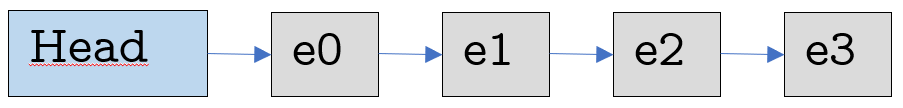
\includegraphics[width=\linewidth]{linked.png}
	
\end{frame}

\subsection{Dubbellänkad lista}

\begin{frame}
	\frametitle{Dubbellänkad lista}
	
	\begin{itemize}
		\item En variant av länkade listor är så kallade dubbellänkade listor
		\item I en dubbelllänkad lista \textit{pekar} alla element på både elementet före och elementet efter
	\end{itemize}
	
	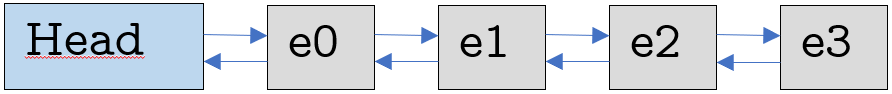
\includegraphics[width=\linewidth]{dubbel.png}
	
\end{frame}

\section{Implementation}


\begin{frame}
	\frametitle{Implementation}

	\begin{itemize}
		\item Listor är väldigt lika köer
		\item Men vill komma åt element inuti
		\item Vill kunna stoppa in element inuti
	\end{itemize}
	
	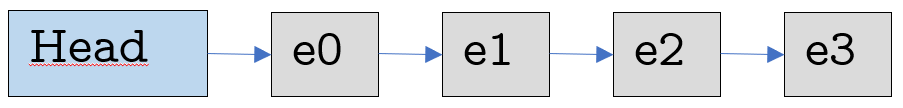
\includegraphics[width=\linewidth]{linked.png}

\end{frame}

\begin{frame}[fragile]
	\frametitle{Implementation}
	\framesubtitle{Komma åt elementet i}
	
	\begin{itemize}
		\item För att komma åt det i:te elementet kan vi loopa typ likadant som för att komma åt det sista
	\end{itemize}
	
	\begin{lstlisting}
METHOD peek(i):
    IF i LESS THAN number of elements
        RAISE IndexError
    SET current TO self.root
    FOR k IN 0 TO i
        SET current TO current.next
    RETURN current.value
	\end{lstlisting}
	
\end{frame}

\section{Övningar}

\begin{frame}[fragile]
	\frametitle{Övning}
	
	\begin{itemize}
		\item Utgå från koden på Classroom och skapa klassen \texttt{LinkedList} utifrån klassdiagrammet nedan:
	\end{itemize}
	
	\begin{center}	
		\begin{tabular}{|c|}
			\hline 
			LinkedList  \\ \hline
			+root: Node\\
			+size: int \\ \hline
			+insert(i:int, value: data) \\
			+peek(): data \\
			+pop(i: int):\\ \hline
		\end{tabular}
	\end{center}
	
\end{frame}

\end{document}